
\documentclass[8pt]{article}
%	options include 12pt or 11pt or 10pt
%	classes include article, report, book, letter, thesis

\usepackage[a4paper,bindingoffset=0.2in,%
            left=0.4in,right=0.6in,top=0.2in,bottom=0.4in,%
            footskip=.15in]{geometry}
            
\usepackage[T1]{fontenc}
\usepackage[polish]{babel}
\usepackage[utf8]{inputenc}
\usepackage{lmodern}
\selectlanguage{polish}
\usepackage{blindtext}
\usepackage{pgfplots}
\usepackage{graphicx}
\usepackage{color,colortbl}

\definecolor{LightCyan}{rgb}{0.97,1,1}
\definecolor{Lightc}{rgb}{1,0.97,1}
\definecolor{Lightcc}{rgb}{1,1,0.97}
\definecolor{Lightccc}{rgb}{0.97,0.97,1}
\definecolor{Lightcccc}{rgb}{1,0.97,0.97}

\title{Algorytmy numeryczne}
\author{Zadanie 4 \\ Tomasz Adamczyk | Aleksander Kosma\\243217 | 238193\\grupa 1 tester-programista}
\date{6 Styczeń 2018}

\begin{document}
\maketitle 

\section*{Aproksymacja}

\subsection*{Gauss-Seidel + struktury danych z biblioteki Eigen}
Przed przystąpieniem do głównego tematu zadania, najpierw należy sprawdzić poprawność wyników nowej metody \textbf{Gaussa-Seidela z wykorzystaniem struktur z biblioteki Eigen}.\\
\\
Przykładowe 3 wyniki z 4 różnych metod w postaci tabeli. Wynikiem odniesienia w tym przypadku jest SparseLU(wnioski z zadania 2). Precyzja metod iteracyjnych została ustawiona na 1E-13 by mieć pewność co do precyzji potrzebnej do głównej części zadania(1E-10).
\begin{center}
 \makebox[\textwidth]{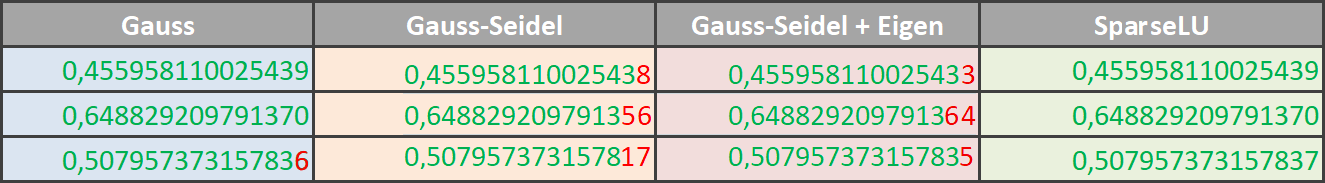
\includegraphics[width=15.5cm,height=2.2cm]{tabela.png}}
\end{center}
Z tych wyników można wysunąć wniosek, że obie implementacje Gaussa-Seidela działają poprawnie.

\section*{Aproksymacja}
\subsection*{Pomiary czasu metod}
Dla głównej części sprawozdania metody iteracyjne liczyły wynik do momentu osiągnięcia precyzji 1E-10. Na wykresie poza metodami, znajduję się też funkcja opisująca czas potrzebny do wygenerowania samego układu macierzy. Wbudowana implementacja Gaussa SparseLU okazuję się być najlepsza.

\begin{center}
 \makebox[\textwidth]{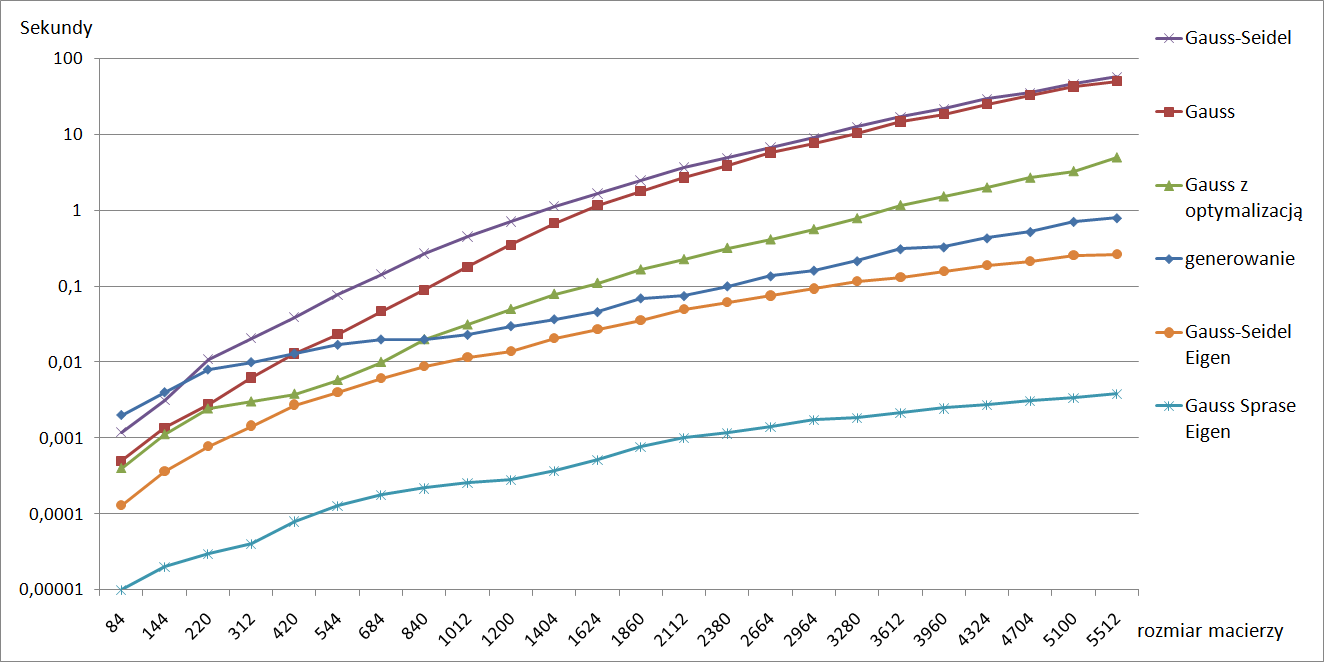
\includegraphics[width=16.5cm,height=9.2cm]{times.png}}
\end{center}

\subsection*{Wielomiany aproksymacyjne}
Zgodnie z nałożonymi z góry stopniami wielomianów, stosując aproksymację średniokwadratową dyskretną, wyliczono następujące funkcje:\\

\renewcommand{\arraystretch}{2}

\begin{tabular}{ | p{3.5cm} | p{12.2cm} | }
  \hline
   \centering Metoda &  \qquad \qquad \qquad \qquad \qquad \qquad \qquad Wzór funkcji \\\hline
  \rowcolor{Lightc}
  Gauss &$F(x)=0,23878 -0,00080121 x+0,00000035354 x^2+0,00000000027256 x^3$ \\\hline
  \rowcolor{LightCyan}
 Gauss z optymalizacją & $F(x)=0,23679-0,00057403x+0,000000240591x^2$\\\hline
 \rowcolor{Lightcc}
   Gauss-Seidel & $F(x)=1,9597-0,005339x+0,000002728x^2$\\\hline
    \rowcolor{Lightccc}
 Gauss Sprase Eigen &$F(x)=-0.000609+0.00000108x$\\\hline
 \rowcolor{Lightcccc}
  Gauss-Seidel Eigen & $F(x)=-0,017882+0,0000207193x$\\\hline
  \hline
\end{tabular}
.\\ \\
Dla poprawy czytelności współczynniki zostały skrócone do 3-5 najistotniejszych wartości.\\
\subsection*{Weryfikacja wyliczonych funkcji}
Wybrane 3 funkcje nałożone na swoje odpowiedniki wyników z metod. Oś pionowa to czas potrzebny do wyliczenia układu, oś pozioma rozmiar wygenerowanej macierzy.


\begin{center}
 \makebox[\textwidth]{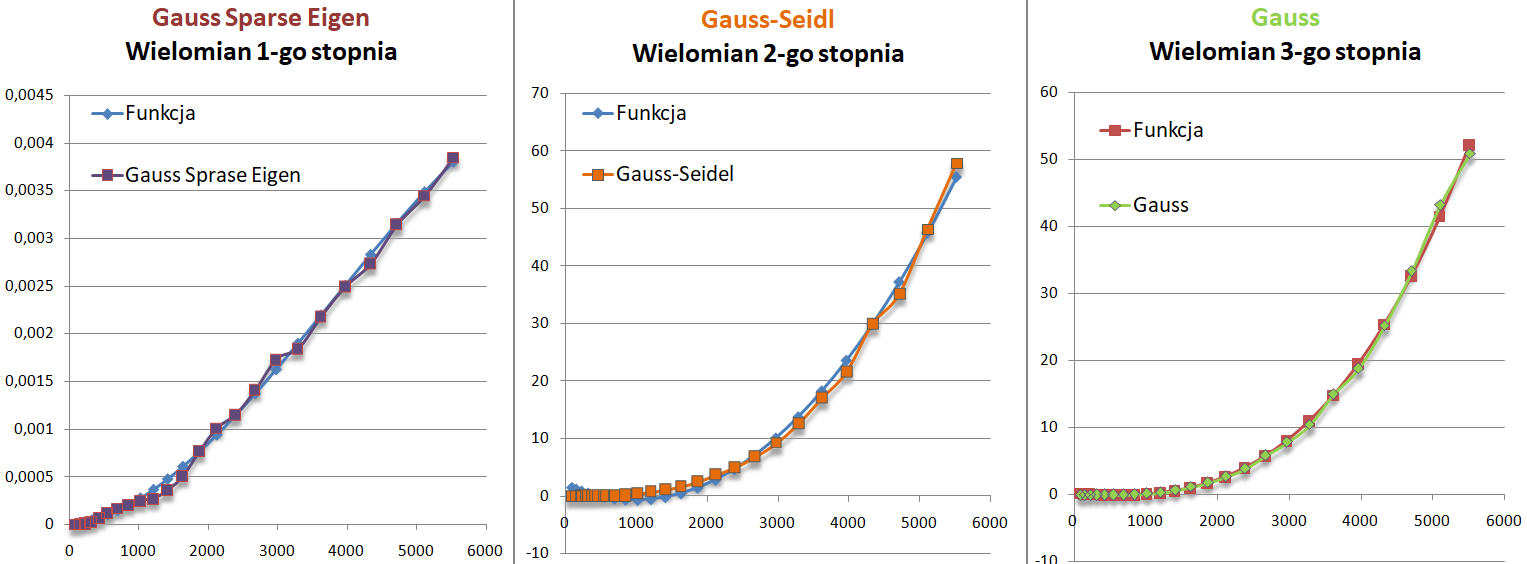
\includegraphics[width=21cm,height=7.5cm]{funkcje.png}}
\end{center}

Nałożenie na siebie funkcji obrazuje dobre odwzorowanie wyliczonych funkcji aproksymacyjnych. Można stwierdzić więc, że wartości wyliczone przez funkcje aproksymacyjne dobrze przybliżają nas do oczekiwanego czasu.

\section*{Extrapolacja}
\begin{center}
\begin{tabular}{ | c | c | c | c | c | }
  \hline
  \multicolumn{5}{|c|}{\textbf{Oczekiwany czas dla rozmiaru macierzy 100 000}} \\
  \hline
  Gauss & Gauss z optymalizacją & Gauss-Seidel &Gauss Sprase Eigen &Gauss-Seidel Eigen \\\hline
  76h & 40min & 7h &0.1sec &2sec \\\hline
  
  \hline
\end{tabular}

\end{center}







\renewcommand{\arraystretch}{1}
\begin{tabular}{ | p{8.2cm} | p{8.2cm} | }
  \hline
  \multicolumn{2}{|c|}{Podział obowiązków} \\
  \hline
  \multicolumn{1}{|c|}{\textbf{Aleksander Kosma} }& \multicolumn{1}{|c|}{\textbf{Tomasz Adamczyk}} \\
  \hline
  -Implementacja Monte Carlo & -Implementacja metod iteracyjnych \\\hline
   -Iteracyjne generowanie układu równań & -Ustalenie i implementacja warunków wygranej \\\hline
    -Szukanie gry bliskiej 50\% & -Wprowadzanie układu równań do macierzy \\\hline
  -Optymalizacja metod iteracyjnych i Gaussa & -Generowanie wyniku poprzez bibliotekę Eigen\\\hline
  -Testy i generowanie wyników & -Napisanie skryptów do generowania wyników \\\hline
  -Obróbka wyników, wykresy i opracowanie & - \\\hline
  
  \hline
\end{tabular}

\end{document}